

\chapter{Developing a Sustainable Platform for Entity Annotation Benchmarks}

%\author{
%Michael Röder \and
%Ricardo Usbeck \and 
%Axel-Cyrille Ngonga Ngomo
%}

%\institute{
%University of Leipzig, Germany\\\email{\{roeder,usbeck,ngonga\}@informatik.uni-leipzig.de}
%}

%\maketitle
%\todo[inline]{Focus on lessons learnt, mention how people can use your software. Accepted development papers will be published in the CEUR-WS workshop proceedings series.}

%\begin{abstract}
The existing entity annotation systems that drive the extraction of RDF from unstructured data are hard to compare as their evaluation relies on different data sets and measures. 
%growing amount of unstructured data on the Document Web and the rising number of tools for structured data from the Web of Data created the need for a growing
%number of entity annotation systems is hard to compare, making it difficult for developers to decide their published experiments are nearly unrepeatable and the diversity of data sets is tremendous.
We developed GERBIL, an evaluation framework for semantic entity annotation that provides developers, end users and researchers with easy-to-use interfaces for the agile, fine-grained and uniform evaluation of 9 annotation tools on 11 different data sets within 6 different experimental settings on 6 different measures. 
In this paper, we present the developed interfaces, data flows and data structures. Moreover, we show how GERBIL supports a better reproducibility and archiving of experimental results.
%Finally, we will explain how to use GERBIL from various perspectives and discuss why this community effort will support semantic annotation research in the long term.
%\end{abstract}


\section{Introduction}
The need for extracting structured data from text has led to the development of a large number of tools dedicated to the extraction of structured data from unstructured data (see~\cite{GERBIL} for an overview).
%The issue of  comparability of results is not to be regarded as being intrinsic to the annotation task.
While these tools do provide evaluation results, these results are rarely fully comparable as they commonly rely on different data sets or different measures. This is partly due to data preparation being a tedious problem in the annotation domain due to the different formats of the gold standards as well as the different data representations across reference data sets.
%These restrictions have led to authors evaluating their approaches on data sets (1) that are available to them and (2) for which writing a parser as well as of (3) an evaluation tool can be carried out with reasonable effort.
%Furthermore, diverse (4) quality measures have been developed and used actively across the annotation research community to evaluate the same task, leading to different results across publications which are not easily comparable. 
Recently, benchmarking frameworks such as the BAT-framework~\cite{cornolti} or NERD-ML~\cite{rizzo2014} for entity annotation systems have began addressing the problem on reproducible experiments for entity annotation.
With GERBIL\footnote{More information and a demo can be found at \url{http://gerbil.aksw.org}} 
 we aim to unify experiment setups, ease implementation and testing effort as well as contribute to an open, repeatable, publishable and archivable open science area to foster an active community of entity annotation tool developers. 

GERBIL goes beyond the state of the art by extending the BAT-framework~\cite{cornolti} as well as Nerd-ML~\cite{rizzo2014} in several dimensions. In particular we provide fine-grained diagnostics for annotation tools, enhanced reproducibility through archiving experiments and assigning URIs to them, easily publishable results by providing results both as RDF (for machines) and tables (for humans).
Overall, we provide the following features:

\textbf{Feature 1: Extensible experiment types.}
An experiment type defines the way used to solve a certain problem when extracting information.
GERBIL extends the six experiment types provided by the BAT framework~\cite{cornolti} (including entity recognition and disambiguation) towards more general, URI based experiments.
%Additionally, we are working on the implementation of an entity typing experiment as it is defined in the Open Knowledge Extraction Challenge 2015\footnote{\url{http://2015.eswc-conferences.org/important-dates/call-OKEC}}.
% as well as it implements 3 experiment types for the Open Knowledge Extraction Challenge 2015\footnote{\url{http://2015.eswc-conferences.org/important-dates/call-OKEC}}.
%\todo[inline]{Micha: Ich finde das nicht so gut, dass wir immer Dinge ins Paper schreiben, die wir noch gar nicht gemacht haben. Wir können gern reinschreiben, dass wir das "Entity Typing" als weiteren Experimenttyp einbringen. Aber mehr haben wir im Moment ja noch gar nicht.}
With this extension, our framework can deal with gold standard data sets and annotators that link to any knowledge base as long as the necessary identifiers are URIs.

\textbf{Feature 2: Matchings.}
GERBIL offers three types of matching between a gold standard and the results of annotation systems: a \emph{strong entity matching} for URIs, as well as a  \emph{strong} and a \emph{weak annotation matching} for entities.

\textbf{Feature 3: Measures.}
Currently, GERBIL offers six measures subdivided into two groups: the micro- and the macro-group of precision, recall and f-measure. As shown in Figure~\ref{cha334:fig:spiderfmeasure}, these results are displayed using interactive spider diagrams that allow the user to easily (1) get an overview of the performance of single tools and (2) compare tools.% with each other.
%and (3) gather diagnostic insights on the performance of tools on particular data sets.

Explicit definitions can be found in Usbeck et al.~\cite{GERBIL}.

\textbf{Feature 4: Diagnostics.}
An important novel feature of our interface is that it displays the correlation between the features of data sets and the performance of tools (see Figure~\ref{cha334:fig:spiderfeature}). By these means, we ensure that developers can easily gain an fine-grained overview of the performance of tools
%w.r.t. a set of features 
and thus detect possible areas of improvement for future work. 



\begin{figure}[htb]
\centering
\subfigure[Example spider diagram of recent A2KB experiments with weak annotation matching.]{
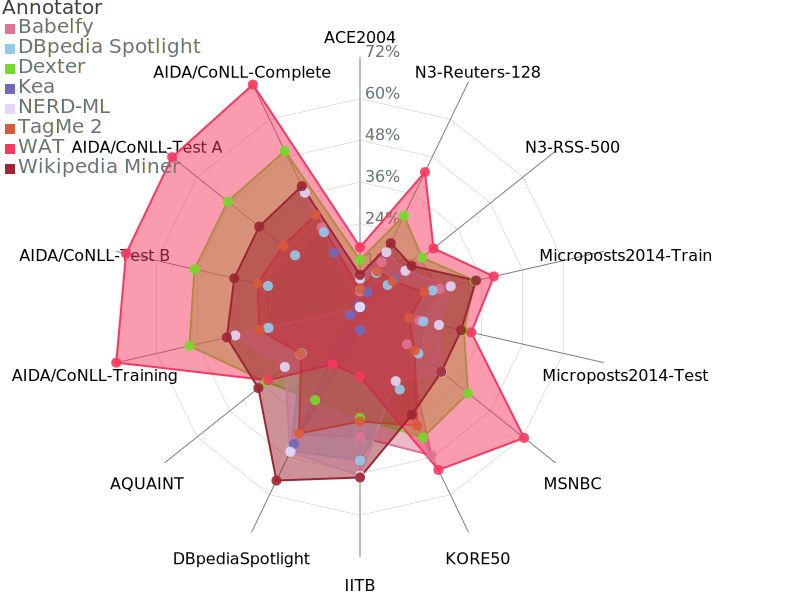
\includegraphics[width=0.48\textwidth]{chapter_three/benchmarking/ESWC_2015_DEV_GERBIL/results.pdf}
\label{cha334:fig:spiderfmeasure}
}~
\subfigure[Spider diagram of correlations between annotation results and data set features.]{
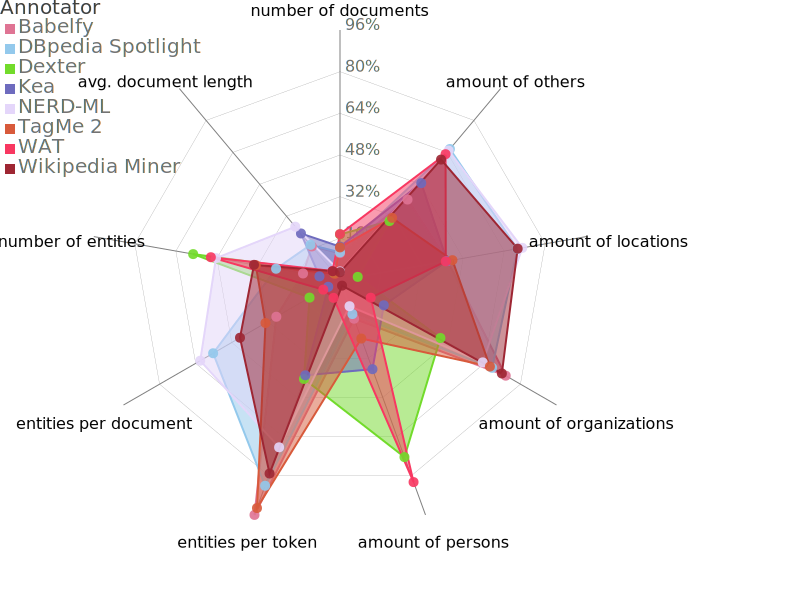
\includegraphics[width=0.48\textwidth]{chapter_three/benchmarking/ESWC_2015_DEV_GERBIL/correlations.pdf}
\label{cha334:fig:spiderfeature}
}
\caption {Spider diagrams generated by the GERBIL interface.}
\end{figure}


\textbf{Feature 5: Annotators.}
Currently, GERBIL offers \overallGERBILannotators entity annotation systems with a variety of features, capabilities and experiments out-of-the-box. 

\textbf{Feature 6: Data sets.}
The latest version of GERBIL offers \overalldatasets data sets.
Thanks to the large number of formats, topics and features of the data sets, GERBIL allows carrying out diverse experiments.

\textbf{Feature 7: Output.}
\label{cha334:sec:output}
GERBIL's experimental output is represented as a table containing the results, as well as embedded JSON-LD\footnote{\url{http://www.w3.org/TR/json-ld/}} RDF data for the sake of archiving experiment results and additional information, e.g., the version of GERBIL that has been used.
Moreover, GERBIL generates a permanent URI for each experimental result.

%To ensure that our framework is useful to both end users and tool developers, its architecture and interface were designed to allow (1) the easy integration of annotators through REST services, (2) the easy integration of data sets via DataHub\footnote{\url{http://datahub.io}} and file uploads, (3) the addition of new performance measures, (4) the provision of diagnostics for tool developers and (5) the portability of results. 

In this paper, we will give a detailed explanation of the different RDF data structures underlying GERBIL's architecture.
We will explain the internal workflow of GERBIL and argue why it simplifies the implementation of further experiments, annotators, data sets, matchings and measures.
%Additionally, we will explain our plans for the longevity of GERBIL as platform for entity annotation systems and 
We conclude by pointing at future work.

%In this paper, we will give a detailed explanation on how the different interfaces are implemented and reason why GERBIL eases the implementation of further annotators, data sets, matchings and measures. % based on the example of the OKE-Challenge.
%We will explain GERBIL's inner dataflow and its importance towards an efficient and scalable experimental platform.
%Furthermore, we will give an in-depth introduction to the underlying RDF data used to described whole experiments and the explain our plans for the longevity of GERBIL as platform for entity annotation systems. 
%Finally, we discuss the impact of design decisions and point towards future work. 


\section{GERBIL's interfaces, dataflow, structure}
\label{cha334:sec:architecture}

\begin{comment}
\subsection{Uses Cases}
Currently, the architecture allows at least three basic use cases: 

\textbf{Repeat already published experiments.}
Compliant with the main goal of GERBIL the reproduction of a certain experiment is central to facilitating research efforts.
Thus, GERBIL offers the opportunity to configure an experiment using four parameters: Experiment type, matching, annotator and data set.
The results will be displayed as table and embedded JSON-LD RDF via a time-stamped URI which can be cited and is stable over time.

\textbf{Run evaluations based on novel data sets.}
GERBIL differentiates three ways of integrating such data sets.
(1) A user can upload a NIF-based corpus (see Section~\ref{cha334:sec:datastructures}) via our web-interface. 
This allows the usage of \emph{closed source} data sets, e.g., business-relevant data or just experimental data not yet ready to be published.
Apart from the experiment results calculated with it, GERBIL will keep \emph{no} other data of such a data set.
(2) GERBIL is able to download NIF-based data sets from \url{datahub.io}.% which will be available after manual revision or
(3) Users can also implement a new data set wrapper source code-wise. 
%While options (1,2) demand knowledge of the NIF format, option (3) uses Java-based wrapper methods to make even legacy data available.
%Furthermore, option (1) allows for the evaluation of \emph{closed source} data set evaluation, e.g., business-relevant data or just experimental data not yet ready to be published.
%Apart from the experiment results calculated with it, GERBIL will keep \emph{no} other data of such a data set.

\textbf{Evaluating a new algorithm.}
Finally, users can submit new webservice-based entity annotation systems in two different ways:
(1) By providing GERBIL with the NIF-based webservice's URI.
This method enables fast prototyping of webservices without the need to implement an annotator wrapper.
To lower barriers, we provide a NIF converter in Java \footnote{\url{https://github.com/AKSW/gerbil/tree/gerbil.nif.transfer}}.
(2) Additionally, a user can use our source code project, implement a new annotator and push his source code back to us. 
%After a feasibility check, we will then bring the enhanced version of GERBIL online and announce via various channels.
%Thus, a tremendous gain with respect to possible comparison opportunities in terms of annotators and data sets is inflicted.
\end{comment}

\subsection{Datastructures}
\label{cha334:sec:datastructures}

GERBIL unifies the different formats used by existing datasets and annotators.
To this end, GERBIL's interfaces are mainly based on the \emph{NLP Interchange Format} (NIF).
This is a RDF-based Linked Data serialization which provides several advantages such as interoperability by standardization or query-ability.
The \emph{NIF-standard} assigns each document an URI as starting point and generates another Linked Data resource per semantic entity.
Each document is a resource of type \texttt{nif:Context} and its content is the literal of its \texttt{nif:isString} predicate. 
Every entity is an own resource with a newly generated URI pointing to the original document via the \texttt{nif:referenceContext} predicate.
Additionally the begin (\url{nif:beginIndex}) and end position (\url{nif:endIndex}) as well as the disambiguated URI (\url{itsrdf:taIdentRef}) and the respective KB (\url{itsrdf:taSource}) are stored.
NIF's paramount position amongst corpora serialisation formats is evident by the growing number of available datasets~\cite{GERBIL}.\footnote{The prefix \texttt{nif} stands for \url{http://persistence.uni-leipzig.org/nlp2rdf/ontologies/nif-core\#} while \texttt{itsrdf} is short for \url{http://www.w3.org/2005/11/its/rdf\#}.}

GERBIL's main aim is to provide comprehensive, reproducible and publishable experiment results.
Thus, GERBIL enforces the use of a machine-readable description for each experiment via JSON-LD\footnote{\url{http://www.w3.org/TR/json-ld/}} RDF data using the RDF DataCube vocabulary~\cite{datacube} next to a human-readable table presentation.
The \emph{RDF DataCube} vocabulary can be used to represent fine-grained multidimensional, statistical data which is compatible with the Linked SDMX~\cite{LinkedSDMX} standard. 
GERBIL models each experiment as \texttt{qb:Dataset} containing \texttt{qb:Observations} for each individual run of a annotator on a dataset.
Each observation features the \url{qb:Dimensions} experiment type, matching type, annotator, corpus, and time. 
The evaluation measures and an error count are expressed as \texttt{qb:Measures}.\footnote{\texttt{qb} is a prefix for for \url{http://purl.org/linked-data/cube\#}.} 

GERBIL relies on the DataID ontology~\cite{dataID} to represent further metadata as well as annotator and corpus information. 
Besides metadata properties like titles, descriptions and authors, the source files of the open datasets themselves are linked as \url{dcat:Distributions}, allowing direct access to the evaluation corpora. 
Furthermore, ODRL license specifications in RDF are linked via \texttt{dc:license}, potentially facilitating automatically adjusted processing of licensed data by NLP tools. 
Licenses are further specified via \texttt{dc:rights}, including citations of the relevant publications.\footnote{The prefix \texttt{dcat} stands for \url{http://www.w3.org/ns/dcat\#} while \texttt{dc} is short for \url{http://purl.org/dc/elements/1.1/}.}
To describe annotators in a similar fashion, we extended DataID for services. 
The class \texttt{Service}, to be described with the same basic properties as dataset, was introduced. 
To link an instance of a \texttt{Service} to its distribution the \texttt{datid:distribution} property was introduced as super property of \texttt{dcat:distribution}, i.e., the specific URI the service can be queried at.
Furthermore, Services can have a number of \texttt{datid:Parameters} and \texttt{datid:Configurations}.
Datasets can be linked via \texttt{datid:input} or \texttt{datid:output}.\footnote{\texttt{datid} is a prefix for for \url{http://dataid.dbpedia.org/ns/core\#}.} 
%Using this detailed description of an experiment opens new research avenues, e.g., tool diagnostics and decision maker support, at the same time as providing provenance information.
%Especially, using RDF as experiment description allows for the extension and adaption of the experimental metadata format on-the-fly.
An example JSON-LD for an archived experiment can be found below.


\scriptsize
%	  \begin{lstlisting}[language=JSON]
\begin{minted}{json}

{
  "@graph" : [ {
    "@id" : "http://gerbil.aksw.org/gerbil/experiment?id=...#experiment_...",
    "@type" : [ "gerbil:Experiment", "qb:Dataset" ],
    "experimentType" : "gerbil:A2KB",
    "matching" : "gerbil:WeakAnnoMatch",
    "structure" : "gerbil:dsd",
    "label" : "Experiment 201503160001"
  }, {
    "@id" : "http://gerbil.aksw.org/gerbil/experiment?id=...#experiment_..._task_0",
    "@type" : "qb:Observation",
    "annotator" : "http://gerbil.aksw.org/gerbil/dataId/corpora/Babelfy",
    "dataset" : "http://gerbil.aksw.org/gerbil/dataId/annotators/ACE2004",
    "statusCode" : "-1",
    "timestamp" : "2015-03-16T12:31:52.469Z"
  } ],
  "@context" : {
    ...
  }
}
\end{minted}
\normalsize

\subsection{Workflow}
\begin{figure}[tb]
    \centering
    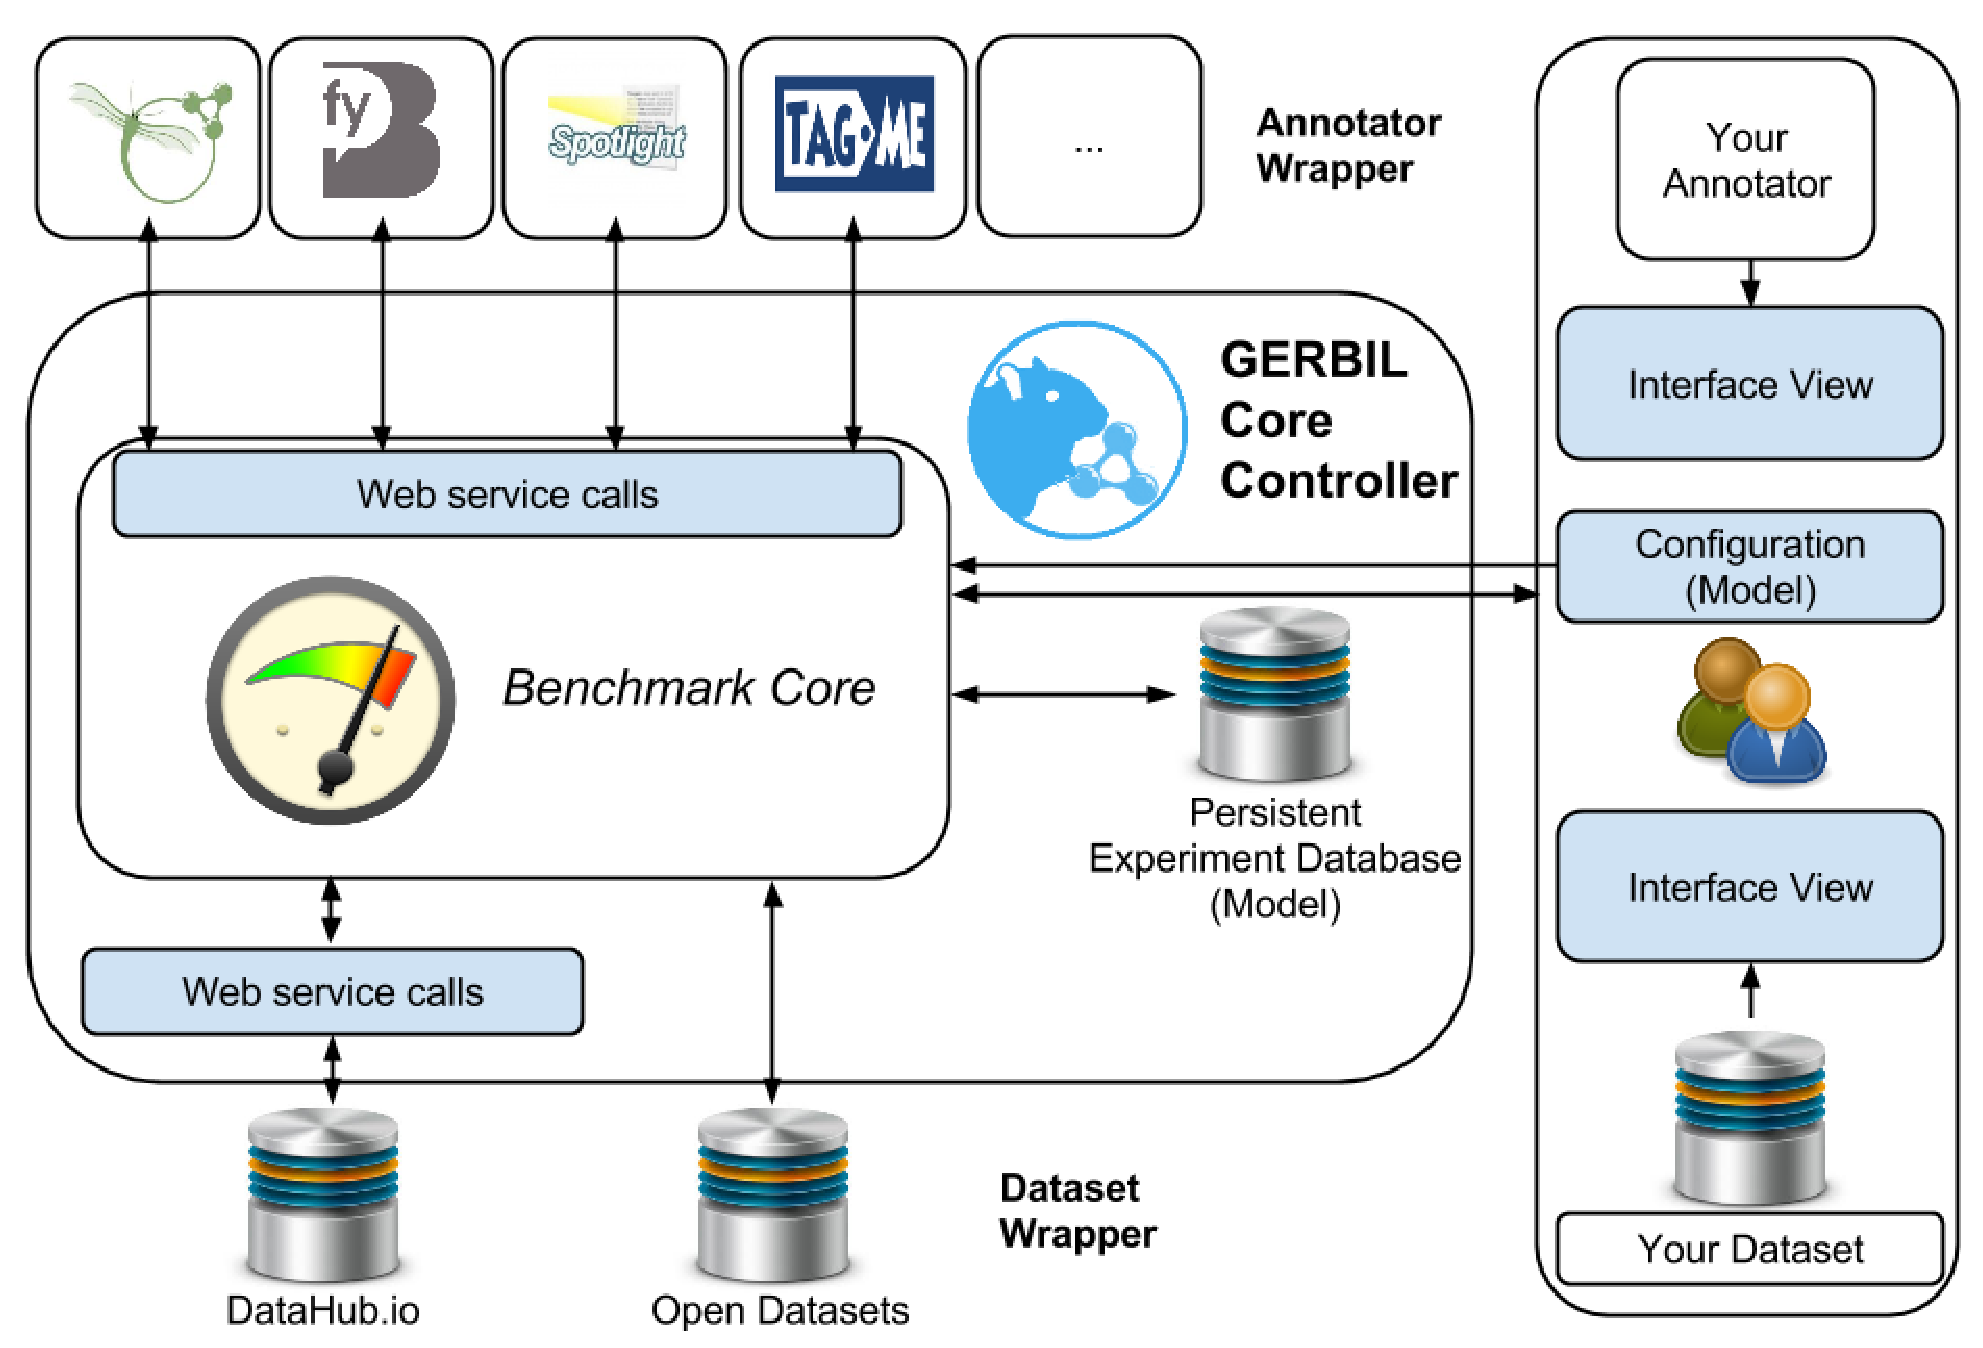
\includegraphics[width=0.9\linewidth]{chapter_three/benchmarking/ESWC_2015_DEV_GERBIL/gerbiloverview.eps}
    \caption{Overview of GERBIL's abstract architecture. Interfaces to users and providers of data sets and annotators are marked in blue.}
    \label{cha334:fig:architecture}
\end{figure}
Figure \ref{cha334:fig:architecture} shows the architecture of GERBIL with the data sets at the bottom, the annotators in the top and the user interface as well as user defined annotator and data set at the right.
A GERBIL session starts at the configuration screen with which a user defines the experiment he is interested in.
Each experiment is divided into tasks.
A task comprises the evaluation of a single annotator using a single data set, is encapsulated into fault-tolerant classes and runs inside an own thread.
Our fault-tolerance classes at two types of errors: (1) an annotator may return error codes for single documents, e.g., because of the missing ability to handle special characters.
While other evaluation frameworks tend to cancel the experiments after an exception thrown by the annotator, GERBIL counts these smaller errors and reports them as part of the evaluation result.
The second type of fault tolerance aims at (2) larger errors, e.g., the data set couldn't be loaded or the annotator is unreachable via its Web service.
These run-time errors are handled by storing one of the predefined error codes inside the experiment database.
Therewith, we ensure that the user gets instant feedback if some parts of the experiment couldn't be performed as expected.

During a task, the single documents of a data set are sent to the annotator.
After finishing the last document, the responses are evaluated.
Currently, the evaluation is focused on the quality, i.e., precision, recall, F1-score and error counts, but can be extended.
Moreover, a runtime is also available~\cite{GERBIL}.
For some experiment types, e.g., the entity-linking tasks, the evaluation needs additional information.
GERBIL is able to search for \texttt{owl:sameAs} links to close the gap between data sets and annotators that are based on different knowledge bases.
Currently, this search is mainly based on the information inside the data set and retrieval of the entity mentioned by the annotator.
The search could be extended by using local search indexes that contain mappings between well-known knowledge bases, e.g., DBpedia and Freebase.
The results are currently written to an HSQL database\footnote{\url{http://hsqldb.org/}}.

\subsection{Extensible Interfaces}

The workflow of GERBIL is very general.
An experiment has a certain experiment type, a matching, and a couple of datasets and annotators.
Thus, it is easily possible to add new experiment types to GERBIL that are not part of the system, e.g., word sense disambiguation.
One major advantage towards this form of extensibility is the usage of NIF for transferring the single documents.
Since NIF is based on RDF the documents sent and received by the system as well as the datasets can be enriched with further information that can be used for the experiments.
Thus, it is easy to add a new experiment type even if the type needs information that cannot be expressed with NIF, e.g., the entity typing task defined in the Open Knowledge Extraction Challenge 2015\footnote{\url{http://2015.eswc-conferences.org/important-dates/call-OKEC}}.
For this challenge, an adapted version of GERBIL has been developed\footnote{\url{https://github.com/AKSW/gerbil/releases/tag/OKE2015}}.
In this version, an annotator that is able to identify the type of a new, unknown entity adds this type to the RDF model of its response.
This information can't be understood directly by the response handling, but is kept and made available to the evaluation component of GERBIL.
Thus, this type information can be used to evaluate the typing performance of an annotator.

%\subsection{Long-term stability}

%Moreover, the research and development unit of the University Leipzig Computation Center will keep daily backups to ensure long-term quotability.

\section{Conclusion and Future Work}
\label{cha334:sec:conclusion}
In this paper, we presented GERBIL, a platform for the evaluation, publishing and archiving of semantic entity annotation experiments.
GERBIL extends the state-of-the-art benchmarks by dealing with data sets and annotators that link to different knowledge bases. 
Furthermore it offers extensible interfaces, reliable experiment descriptions as well as diagnostics and decision support.
Our future work will comprise a better experiment task scheduling to achieve a higher efficiency. 
%GEBRIL has a high potential to save memory if the experiment tasks could share their common elements, e.g., the data sets they are working on.
Another task is the improvement of the user interface towards a better intelligibility.
Finally, we will devise a solution to ensure that GERBIL remains available to the community for the years to come.

%As GERBIL is still a young project and thus we are trying to explore the borders of our endeavour. 
%As GERBIL has been launched within several PhD projects funded by European Social Fund and several other European and German research grants the deployment of GERBIL is safeguarded within the next five years.
%Furthermore, we have two fallback solutions: (1) the research group AKSW and the university computing center which currently already hosts more than 30 open source projects announced a strong partnership with the GERBIL platform.
%(2) GERBIL is open source software which can be maintained and hosted by anybody.

%\bibliographystyle{abbrv}
%\bibliography{myrefs}


%\end{document}